\section{Overview of the System}
This chapter consists of the general introduction, the study of the existing system, requirement specification and system design. The study of the existing system includes main findings from interviews, requirements specifications include functional, non-functional requirements, software and hardware requirements. System design comprises modelling the solution from the findings.


\section{System study}
The data gathered using the selected data collection techniques enabled the system developers to garner information which was studied to realise the weaknesses of the existing systems and how the new system would be designed in a better way.


\section{Study of the existing system}
Our case study as previously mentioned was the Makerere University Parking System. We conducted two interviews with the project manager who informed us all the details of the current system and its shortcomings. Some details however such as average revenue garnered by the system,etc. were not shared with us for confidentiality purposes.


\section{System Analysis}

\subsection{Data Analysis}
Below is a summary of some of the main findings from the survey we conducted.

\subsubsection{Breakdown of the intended users of the existing and proposed system}
Our analysis found that the main users of the system are fall into two categories, each with its own subcategories. These are:
\begin{itemize}
    \item Frequent users: This comprises users students, lecturers and university staff who are the main users of the system.
    \item Occasional users: This comprises visitors to the university or ordinary passers-by who wish to use the system quickly perhaps a shortcut to avoid traffic, or a brief visit to the university, among other reasons
\end{itemize}
The system therefore ought to have a way to discern between these two categories, and frequent users are not expected to make payments while non-frequent users do


\begin{figure}[h]
    \hspace{-3cm}
    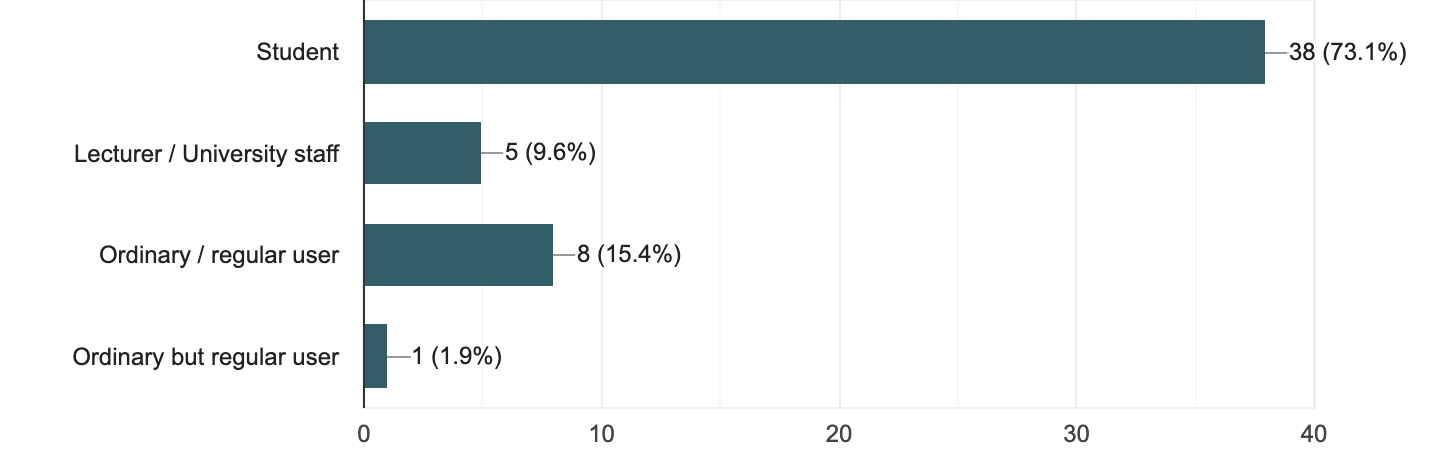
\includegraphics[scale = 0.7]{images/users}
    \caption{Breakdown of intended users of the system}
\end{figure}

\clearpage

\subsubsection{Analysis of frequency of usage of the current system}
We were also able to analyse the frequency of usage of the current system. We found that the majority of our respondents use the system on a daily basis, with a few using it on a weekly basis. This is expected since the main users of the system are students, lecturers and university staff who are expected to be at the university on a daily basis. The occasional users are expected to be a minority.


\begin{figure}[h]
    \begin{center}
        \hspace{-7cm}
        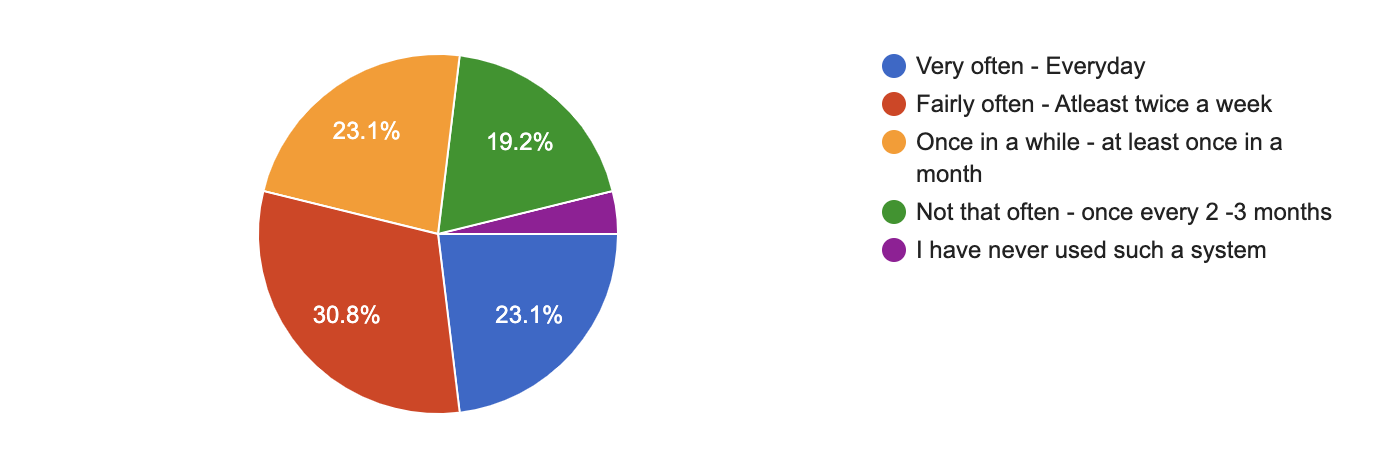
\includegraphics[scale = 0.8]{images/usage}
        \caption{Respondents' frequency of usage of the current system}
    \end{center}
\end{figure}

\clearpage

\subsubsection{Familiarity with local mobile payment platforms}
We believe one of the benefits of our proposed system is that we leverage local mobile money platforms such as MTN Mobile Money and Airtel Money. We therefore sought to find out how familiar our respondents were with these platforms. We found that the majority of our respondents were familiar with these platforms, with a few not being familiar with them. This is expected since mobile money is a popular payment platform in Uganda.


\begin{figure}[h]
    \begin{center}
        \hspace{-3cm}
        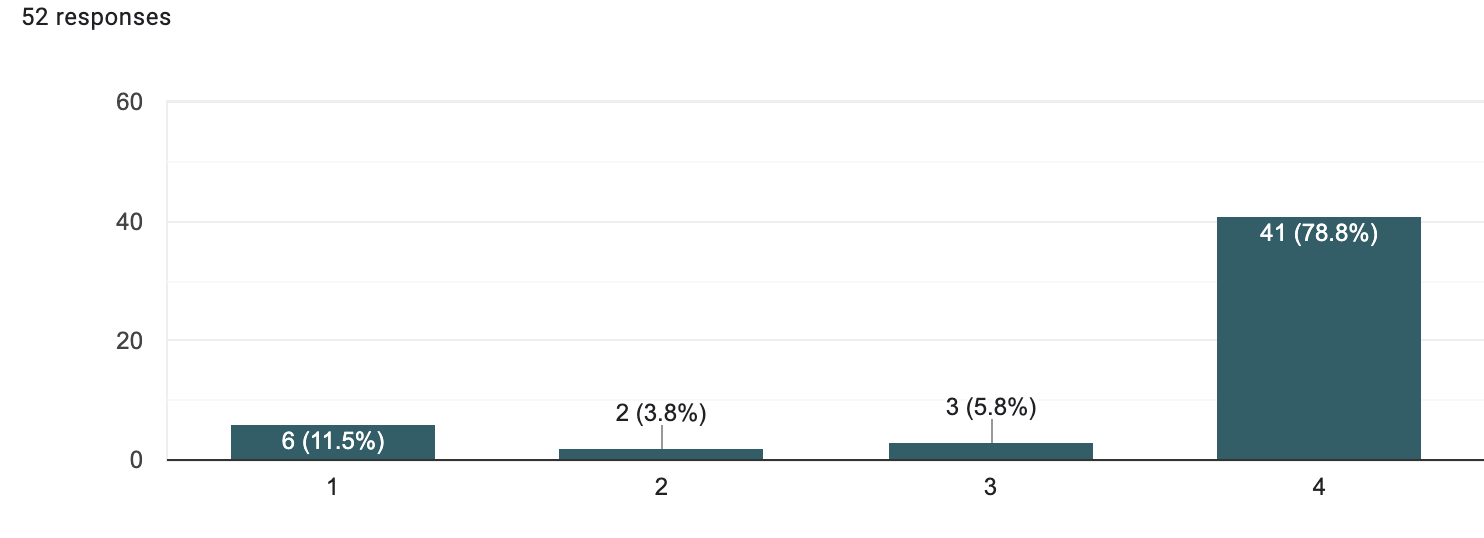
\includegraphics[scale = 0.5]{images/mob-mon}
        \caption{Respondents' familiarity with mobile money platforms on a scale of 1 to 5}
    \end{center}
\end{figure}

\clearpage

\subsubsection{Level of satisfaction with existing system}

We also sought to find out how satisfied our respondents were with the existing system. We found that the majority of our respondents were either not satisfied or fairly satisfied with the existing system, with a few being satisfied with it. This is expected since the existing system has a number of shortcomings which we have already highlighted.

\begin{figure}[h]
    \begin{center}
        \hspace{-3cm}
        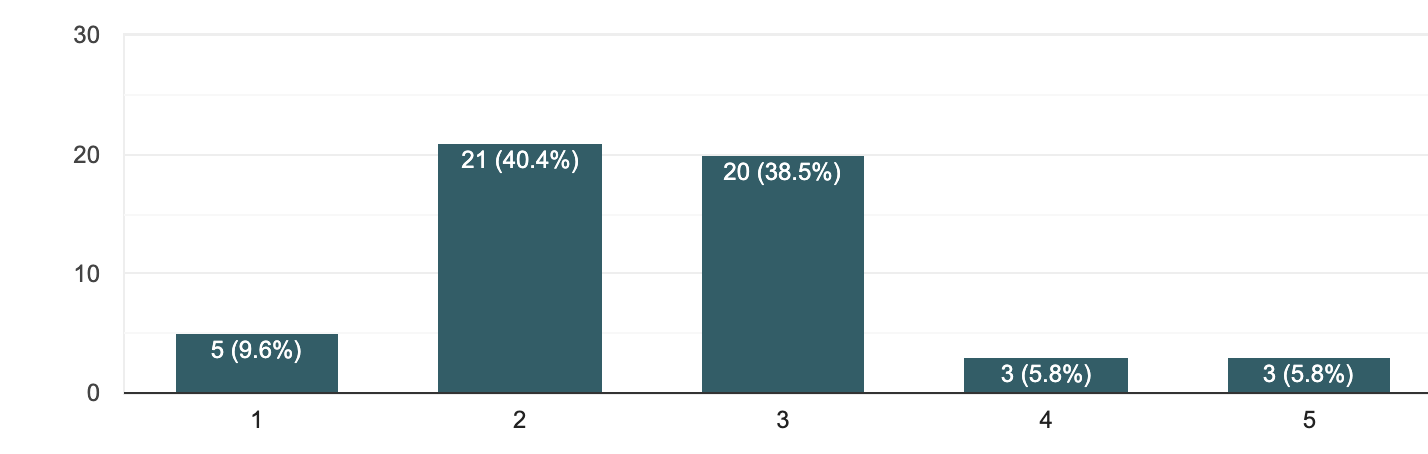
\includegraphics[scale = 0.5]{images/satisfaction}
        \caption{Respondents' level of satisfaction with the existing system on a scale of 1 to 5}
    \end{center}
\end{figure}

\clearpage

\subsubsection{Frequency of encountering challenges with the existing system}
We also sought to find out how often our respondents experienced problems such as malfunction of the ticketing machine, difficulty finding the payment points. We found that the majority of our respondents experienced problems with the existing system occasionally, others frequently and a few never experienced problems with the existing system.

\begin{figure}[h]
    \begin{center}
        \hspace{-3cm}
        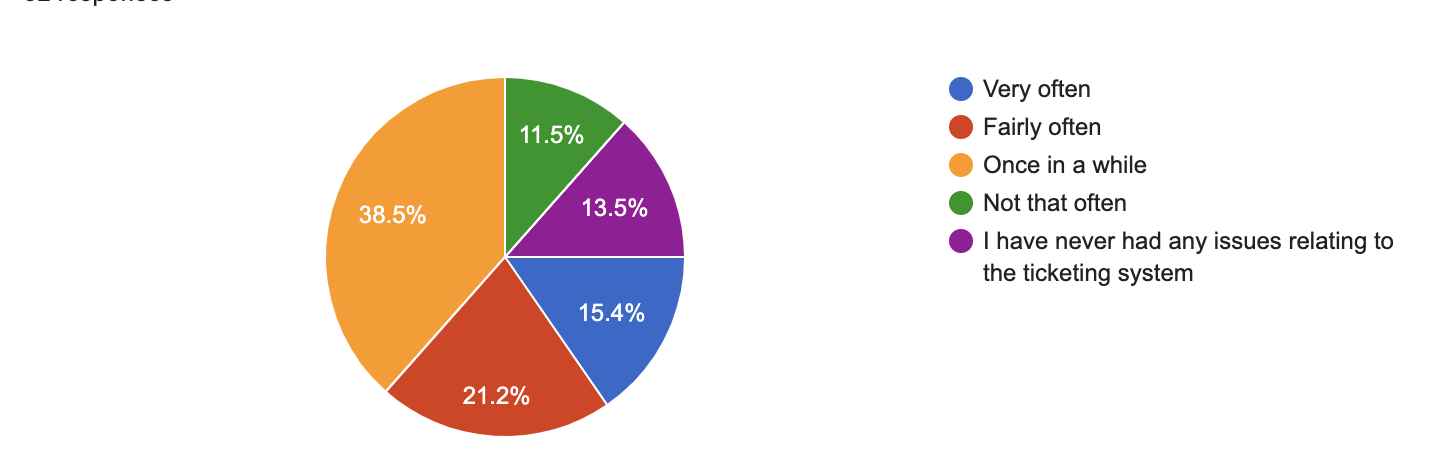
\includegraphics[scale = 0.6]{images/prob-freq}
        \caption{Respondents' frequency of encountering problems with the existing system}
    \end{center}
\end{figure}

\subsubsection{Opinion on the hefty fine for losing a ticket}
The researchers also sought from the respondents their individual opinions on the hefty fine for losing a ticket. All respondents expressed dissatisfaction with the idea, justifying the need for a digital alternative of ticketing that avoid such scenarios.

\clearpage

\subsection{Requirements Specification}
In order to come up with the end user requirements for the new system, data was collected through interviews with both the project manager of the current system at Makerere University and a survey shared with motorists who use the gates.

The collected data was then analysed in order to come up with the requirements of the new system. This section included the requirements of the new system divided into user requirements and system requirements.

\subsubsection{User Requirements}
This encompasses the requirements of the system from the user’s point of view.

The users identified are gate attendants who can also double as administrators of the system as well as motorists who use the gates. The motorists are split into two further categories: regular users and occasional users.
\begin{itemize}
    \item \textbf{Gate attendants / Administrators}: Manages the ETolls System
    \item \textbf{Motorists}: Uses the ETolls System to make their payment
\end{itemize}

\subsubsection{Functional Requirements}
This is to with the services that the system will provide to the users. The system will be able to:
\begin{itemize}
    \item Allow new users(motorists) to register for the system
    \item Allow registered users to log in to the system
    \item Allow users to make payments for parking
    \item Allow users to view their payment history
    \item Allow users to view their parking history
    \item Allow the system administrator to add or delete users
\end{itemize}

\subsubsection{Non-Functional Requirements}
These are requirements that are not directly related to the functionality of the system but are important for the system to work properly. These include:
\begin{itemize}
    \item The system should allow for easy registration of users
    \item The system should support various payment platforms such as MTN Mobile Money, Airtel Money
    \item The system should be secure
    \item The system verifies all user inputs and users must be notified in case of error
\end{itemize}

\subsection{System Design}
This section defines the physical architectural design and the logical design (showing processes, sub processes and data flows to/from external entities) and database design of the system required to satisfy the specified requirements.

\subsubsection{Architectural Design}
An architecture diagram is a representation of elements that comprise a given system\cite{tilley2019systems}.

The system will comprise a mobile application as well as remote server hosted on the cloud. The mobile application will be used by the motorists to make payments and view their payment history. The remote server will be used to store the data of the users and their payment history. The final component is the microcontroller which will be used to control the gates and communicate with the remote server.

For demonstration purposes, the system will be demonstrated using a microcontroller and a servo motor to demonstrate the logic of opening and closing of gates


\begin{figure}[h]
    \begin{center}
        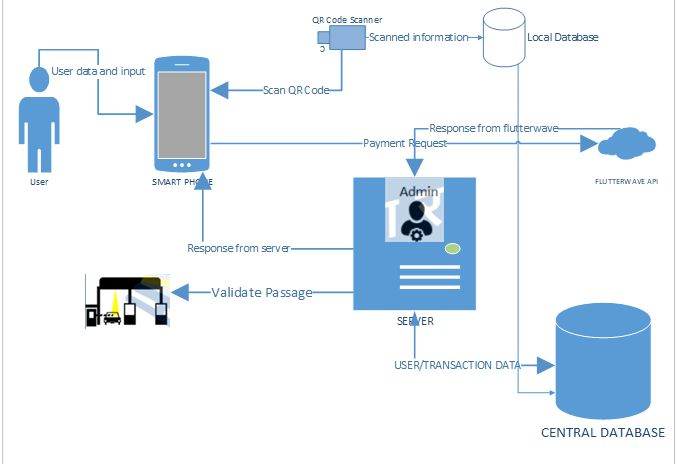
\includegraphics[scale = 0.8]{images/etolssys}
        \caption{System Architecture diagram for E-Tolls System}
    \end{center}
\end{figure}

\clearpage

\clearpage

\subsubsection{Use case diagram}
A use case diagram is a graphical representation of a given user's possible interactions with a system. It gives broad view of a system and the different types of users and use cases within that system \cite{alhir2003learning}.
Below is a use case diagram for our proposed system
\begin{figure}[h]
    \begin{center}
        \hspace{-2cm}
        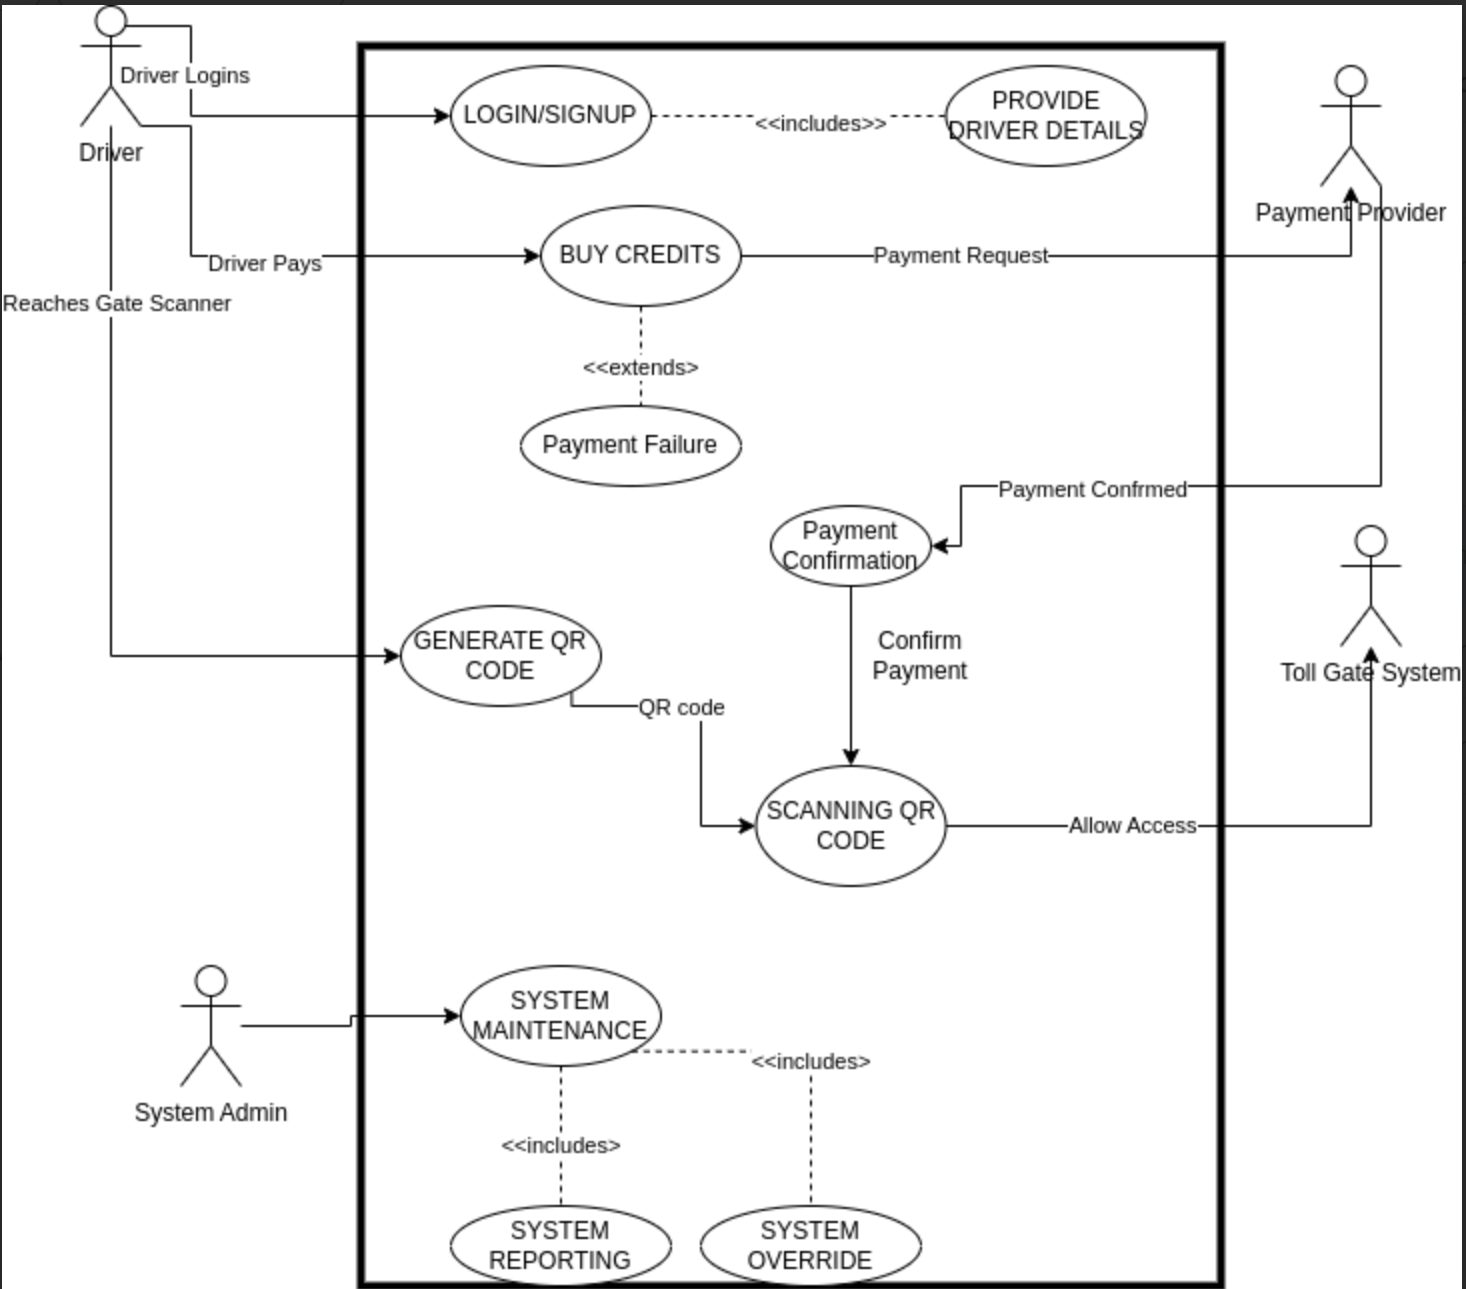
\includegraphics[scale = 0.6]{images/use case diagram}
        \caption{Use Case diagram for E-Tolls System}
    \end{center}
\end{figure}

\clearpage

\subsubsection{Entity Relationship Diagram}
An entity relationship diagram (ERD), also known as an entity relationship model, is a graphical representation that depicts relationships among people, objects, places, concepts or events within a system. The diagram below shows the entities and their relationships in our system\cite{bagui2012database}.
\begin{figure}[h]
    \begin{center}
        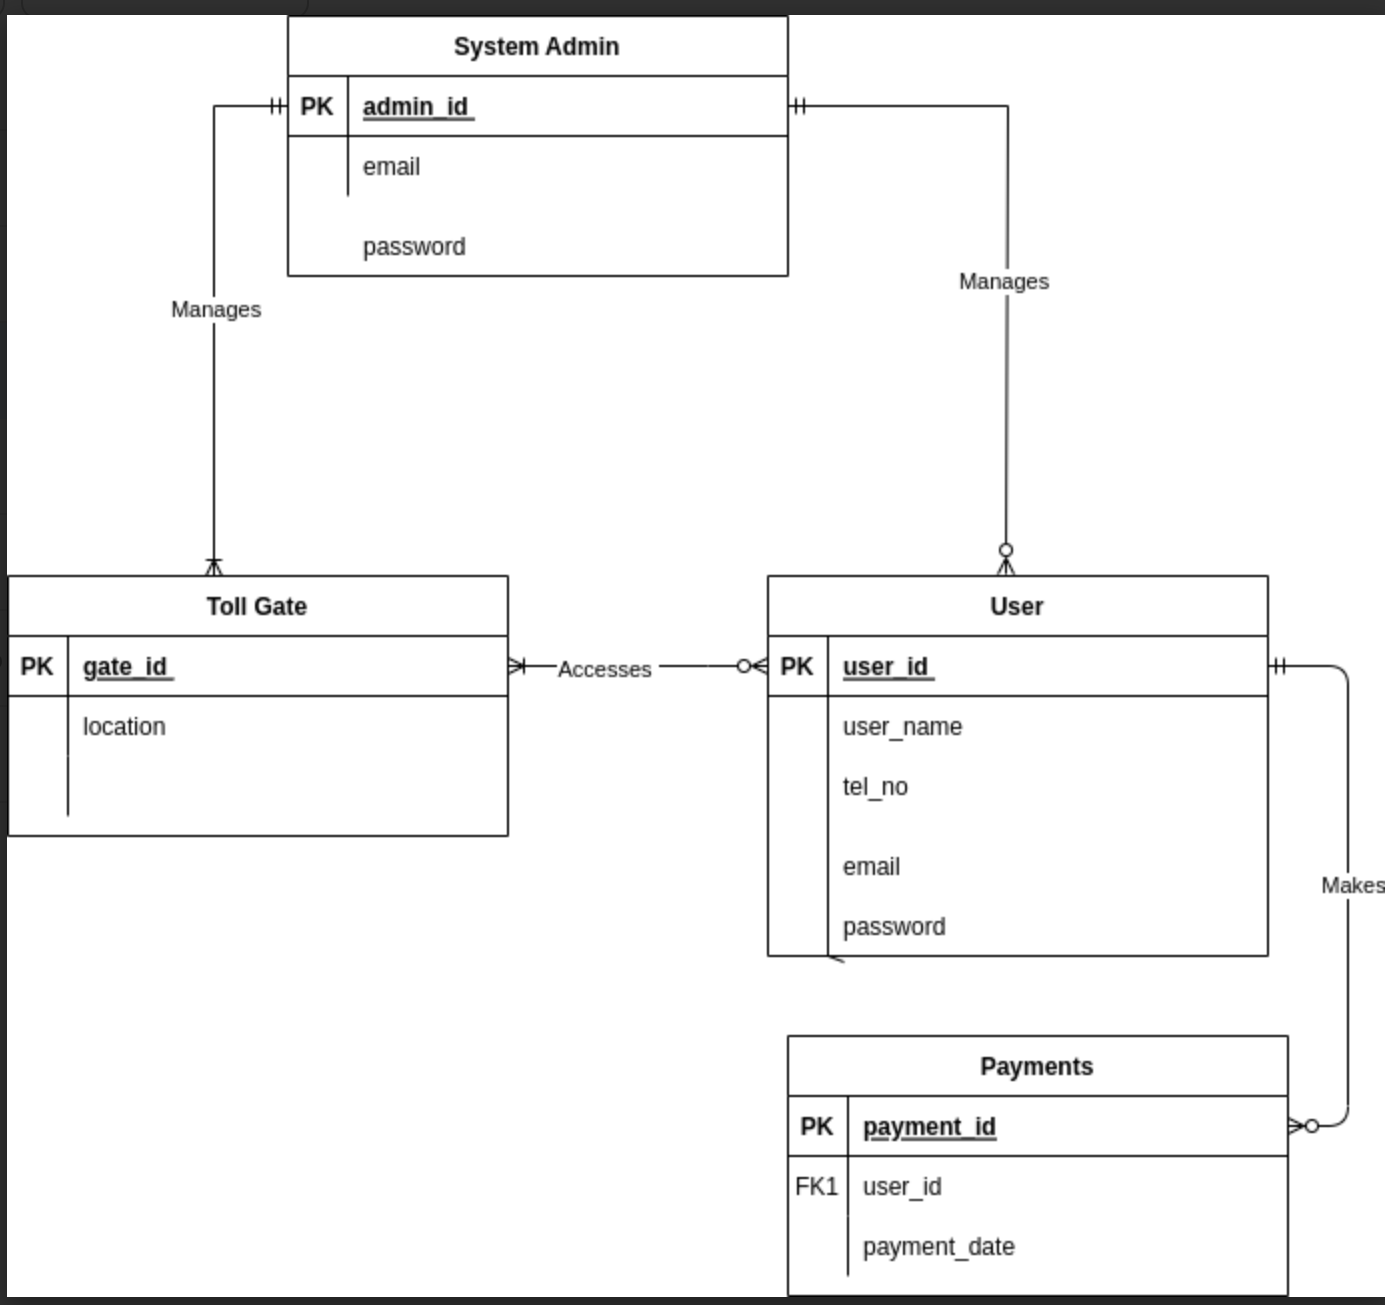
\includegraphics[scale = 0.6]{images/erd}
        \caption{Entity Relationship Diagram for E-Tolls System}
    \end{center}
\end{figure}


\clearpage

\subsubsection{Flow chart}
The flow chart represents the dynamic behavior of the objects and classes that have been identified as part of the system. The flow chart helped us describe the plan in order to perform the different tasks. It showed what was done when the decision was made and when to go to each process as a result. The flow chart helped us build a step-by-step picture of the processes of our system.
\begin{figure}[h]
    \begin{center}
        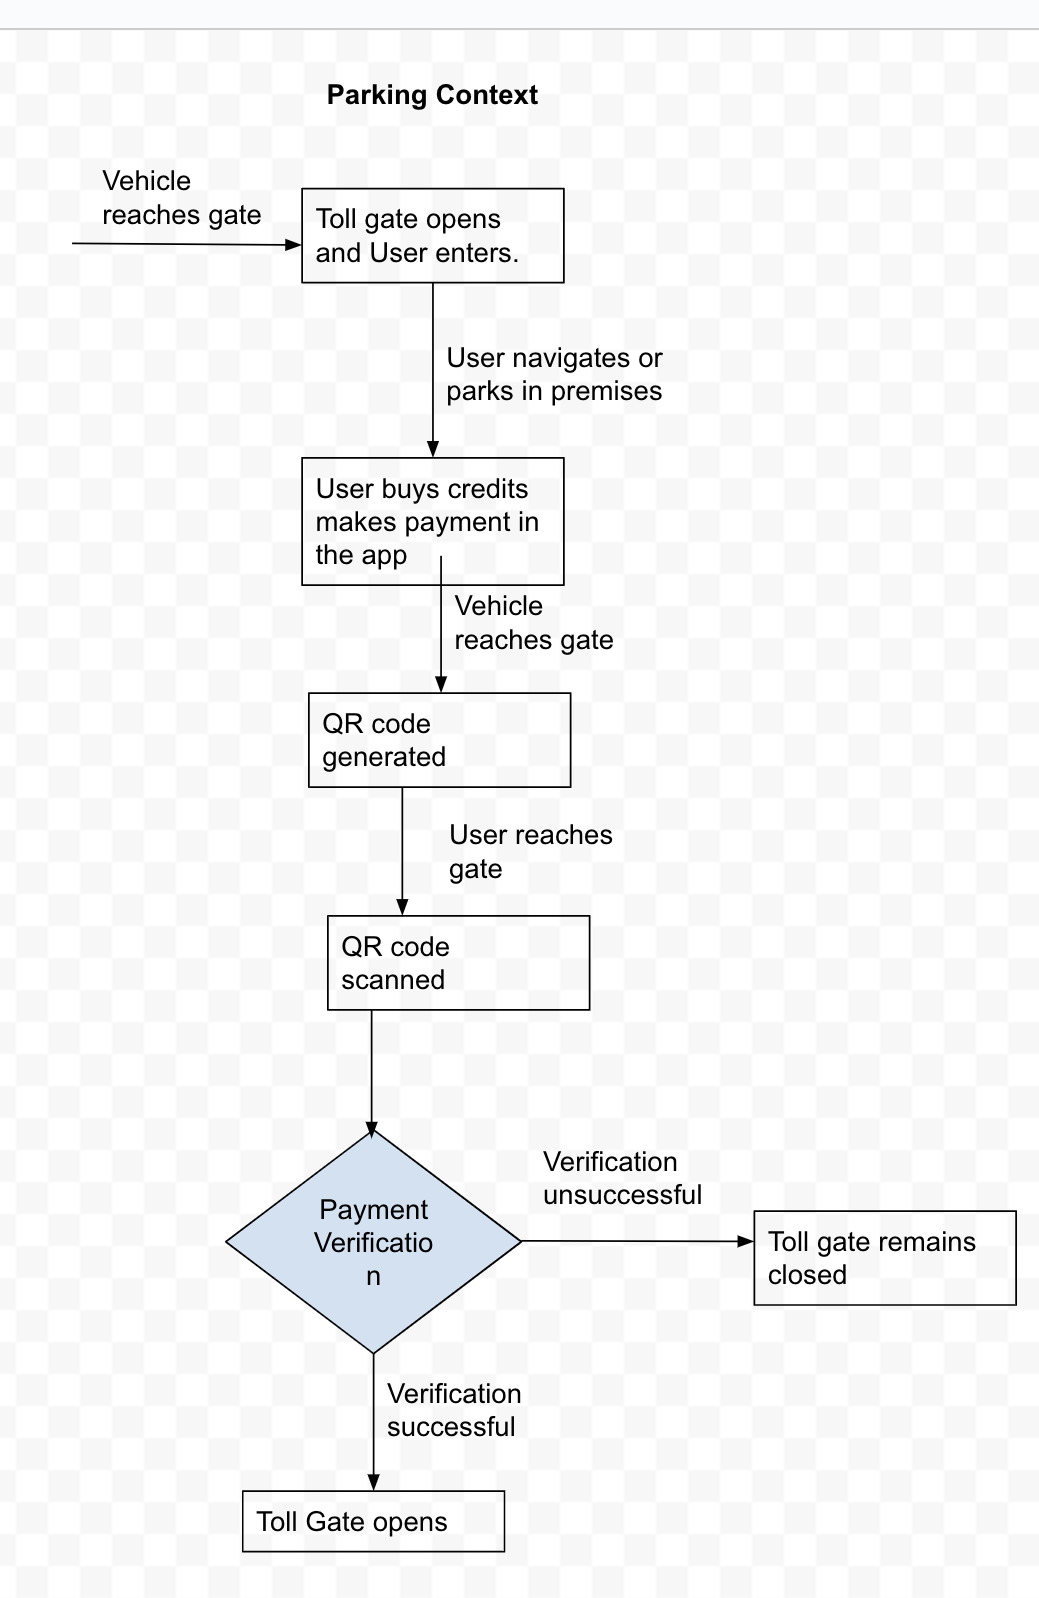
\includegraphics[scale = 0.6]{images/userflowdiagram}
        \caption{System Architecture diagram for E-Tolls System}
    \end{center}
\end{figure}
\clearpage

\subsubsection{Context Diagram}
A context diagram is a visual representation of how external elements interact with a system, such as a project or a software system. It clarifies the interfaces and boundaries of the project or process at hand, and shows the project’s interactions with other systems and users\cite{wysocki2006effective}.

\begin{figure}[h]
    \begin{center}
        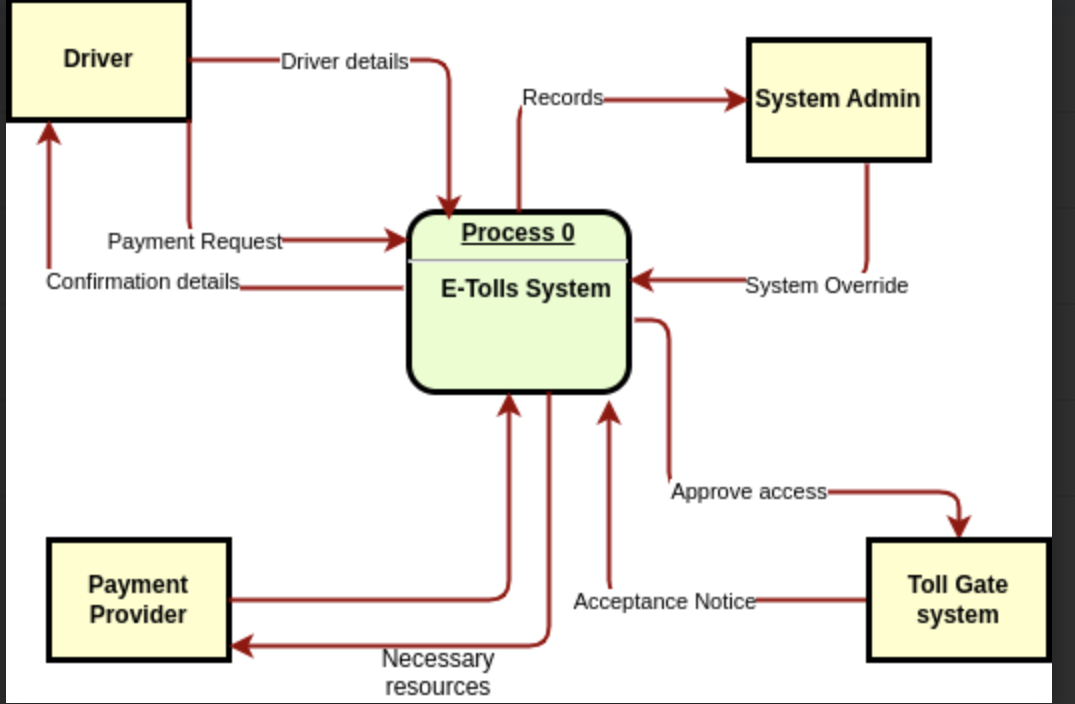
\includegraphics[scale = 0.6]{images/context_diagram}
        \caption{Context Diagram for E-Tolls System}
    \end{center}
\end{figure}